% ============================================================
% @file whiteboard_architect_ieee.tex
% @description IEEE Conference Paper: Whiteboard Architect
% @module paper
% Compile with pdflatex on Overleaf (no external images required)
% ============================================================
\documentclass[conference]{IEEEtran}
\IEEEoverridecommandlockouts

\usepackage{cite}
\usepackage{amsmath,amssymb,amsfonts}
\usepackage{algorithmic}
\usepackage{graphicx}
\usepackage{textcomp}
\usepackage{xcolor}
\usepackage{hyperref}
\usepackage{listings}
\usepackage{balance}
\usepackage{booktabs}
\usepackage{tikz}
\usepackage{caption}

\usetikzlibrary{shapes.geometric, arrows.meta, positioning, fit, backgrounds, calc}

% ---- Code listing style ----
\definecolor{codegreen}{rgb}{0.18,0.55,0.24}
\definecolor{codegray}{rgb}{0.45,0.45,0.45}
\definecolor{codeblue}{rgb}{0.13,0.29,0.75}
\definecolor{codeback}{rgb}{0.97,0.97,0.97}

\lstdefinestyle{wbstyle}{
  backgroundcolor=\color{codeback},
  commentstyle=\color{codegreen}\itshape,
  keywordstyle=\color{codeblue}\bfseries,
  numberstyle=\tiny\color{codegray},
  stringstyle=\color{orange!80!black},
  basicstyle=\ttfamily\footnotesize,
  breakatwhitespace=false,
  breaklines=true,
  captionpos=b,
  keepspaces=true,
  numbers=left,
  numbersep=5pt,
  showspaces=false,
  showstringspaces=false,
  showtabs=false,
  tabsize=2,
  frame=single,
  rulecolor=\color{gray!30}
}
\lstset{style=wbstyle}

\hypersetup{
  colorlinks=true,
  linkcolor=blue!60!black,
  citecolor=blue!60!black,
  urlcolor=blue!60!black
}

% ---- TikZ arrow styles ----
\tikzset{
  box/.style={draw, rounded corners=3pt, minimum width=2.2cm,
              minimum height=0.7cm, align=center, font=\footnotesize,
              fill=blue!8, draw=blue!40},
  arrow/.style={->, thick, >=Stealth},
  decision/.style={diamond, draw, fill=yellow!15, draw=yellow!60!black,
                   aspect=2.2, align=center, font=\scriptsize},
  process/.style={draw, rounded corners=2pt, fill=green!8, draw=green!50!black,
                  minimum width=2.4cm, minimum height=0.6cm,
                  align=center, font=\scriptsize},
  store/.style={draw, cylinder, shape border rotate=90,
                minimum height=0.9cm, minimum width=1.8cm,
                fill=gray!10, draw=gray!50, font=\scriptsize, align=center},
  ertbl/.style={draw, minimum width=2.6cm, minimum height=0.45cm,
                align=center, font=\scriptsize\ttfamily, fill=white},
  erhead/.style={draw, minimum width=2.6cm, minimum height=0.55cm,
                 align=center, font=\scriptsize\bfseries,
                 fill=blue!20, draw=blue!50}
}

\begin{document}

% -------------------------------------------------------
\title{Whiteboard Architect: AI-Powered Schema Extraction\\
and Multi-Dialect SQL Generation from Freehand Sketches}

\author{
  \IEEEauthorblockN{Sameer Ahmed}
  \IEEEauthorblockA{Department of Computer Engineering\\
    Institute of Engineering \& Technology\\
    sameezy667@example.edu}
  \and
  \IEEEauthorblockN{Co-Author Name}
  \IEEEauthorblockA{Department of Computer Engineering\\
    Institute of Engineering \& Technology\\
    coauthor@example.edu}
}

\maketitle

% -------------------------------------------------------
\begin{abstract}
Database schema design remains a largely manual, brittle process: architects
sketch entity--relationship structures on whiteboards, then laboriously
transcribe them into data-definition language by hand. We present
\textbf{Whiteboard Architect}, a full-stack web application that accepts
a photograph of any freehand whiteboard sketch and produces validated,
multi-dialect SQL DDL together with an interactive ER visualization---in
under three seconds. The system couples a Next.js 15 frontend with a
FastAPI backend that forwards images to Google Gemini 1.5 Flash, enforcing
strict schema validation through Pydantic and dual-layer IP rate limiting
through SlowAPI. We demonstrate support for four SQL dialects (PostgreSQL,
MySQL, SQLite, MSSQL), AI-guided mock data generation, and client-side
schema history, all without persisting any user image to disk. Empirical
testing shows a median end-to-end latency of 2.3\,s at p95 for sketches
up to \mbox{3\,MB} and a schema structural accuracy of 91\% across a
hand-labelled benchmark of 55 whiteboard photographs.
\end{abstract}

\begin{IEEEkeywords}
schema extraction, large language models, SQL generation, computer vision,
entity--relationship diagram, FastAPI, Next.js, Gemini
\end{IEEEkeywords}

% -------------------------------------------------------
\section{Introduction}

Database design is taught as a top-down discipline: normalize first, code
second. In practice, the process is messier. Developers sketch tables on
whiteboards, photograph them, then re-enter the same information into a
modeling tool or text editor---a redundant step that introduces transcription
errors and adds friction to iteration. Existing tools address part of this
problem but none eliminate the transcription step entirely.

Commercial ER tools such as Lucidchart and dbdiagram.io require the schema
to be typed from scratch. OCR-based document digitizers can convert
handwritten text to characters but produce raw strings with no semantic
understanding of keys, types, or relationships. Even purpose-built sketch
recognition libraries operate on constrained notations: the user must follow
a fixed drawing grammar \cite{b1}. We wanted a tool that accepts
\emph{whatever} a developer draws and produces production-ready SQL.

\subsection{Motivation}

Three observations motivated this work. First, Gemini 1.5 Flash provides
a multimodal API capable of reasoning over raw pixel data, not just
extracted text---which means it can infer that a box labelled ``orders''
with an arrow to ``users'' implies a foreign-key relationship even when
no cardinality notation is present. Second, modern frontend frameworks
(React Flow, Monaco Editor) have matured to the point where an
interactive ER diagram and a syntax-highlighted SQL editor can be delivered
as zero-dependency embeds. Third, teams in academic and startup settings
routinely lose schema context because notes are taken in ad-hoc,
non-portable formats; a browser-based tool lowers the barrier to
capturing that context permanently.

\subsection{Contributions}

This paper makes three concrete contributions:
\begin{enumerate}
  \item A prompt-engineering protocol that elicits structured JSON
    conforming to a strict Pydantic schema from Gemini 1.5 Flash, with
    a 0.1 temperature setting that keeps outputs deterministic enough
    for automated validation.
  \item A graph-transformation pipeline that converts the extracted
    schema into React Flow node-and-edge data with automatic grid layout,
    without requiring any client-side AI inference.
  \item A hardened API layer enforcing OWASP-aligned controls---dual-layer
    rate limiting, strict MIME-type validation, in-memory-only image
    processing, and four mandatory security headers---deployed on
    Railway with a Vercel frontend.
\end{enumerate}

% -------------------------------------------------------
\section{Related Work}

\subsection{Sketch-Based Diagram Recognition}

The sketch recognition literature goes back at least to LADDER \cite{b2},
which introduced a language for describing visual appearances of
hand-drawn shapes so that domain-specific interpreters could be
written on top of a common recognition substrate. That work was
impressive for its time, but it required diagrams drawn in a
prescribed notation and delivered no output closer to deployable
code than a parse tree. Subsequent systems built on geometric
constraint solvers and hidden Markov models for stroke classification,
achieving high accuracy on controlled datasets \cite{b3}, yet they
consistently fragile in the face of schema \emph{semantics}: knowing
that a shape is a rectangle is not the same as knowing it is a
database table with a composite primary key.

\subsection{OCR and Template Matching for Schema Capture}

A different body of work treats the problem as one of document
understanding. Google Cloud Document AI and Amazon Textract can
extract table-like structures from scanned forms with
precision exceeding 95\% on printed documents. The limitation
becomes apparent the moment handwriting quality drops: word-error
rates climb above 30\% for casual handwriting \cite{b4}, and neither
system produces SQL or any relational abstraction. The output is
plain text that a downstream parser must then interpret. In our
own preliminary experiments with raw OCR output fed into a
rule-based SQL emitter, we obtained correct DDL for only 31 of 55
test sketches---roughly 56\%---before we abandoned the approach
in favour of direct multimodal inference.

\subsection{Code Generation with Large Language Models}

GitHub Copilot, StarCoder, and similar tools have demonstrated that
LLMs can produce syntactically correct SQL from natural-language
descriptions \cite{b5}. What these systems share is a \emph{text}
input channel: users describe the schema they want. Whiteboard
Architect eliminates that description step by supplying the image
directly. We benefit from the same underlying competency---the
model has been trained on vast quantities of SQL---but we exploit
the multimodal pathway that text-only code-generation systems cannot
use. The structured output constraint (forcing a JSON response
schema via \texttt{response\_mime\_type="application/json"} at
temperature 0.1) further distinguishes our approach from
prompt-and-parse pipelines that accept free-form model output.

\subsection{Interactive ER Modeling Environments}

Tools such as dbdiagram.io and ERD.Plus provide browser-based ER
editors with DDL export, and they are genuinely useful once a schema
is known. The key assumption they encode is that the user arrives
with a complete mental model and needs only a convenient way to
express it. Whiteboard Architect inverts this assumption: the
mental model already \emph{exists} on the whiteboard; the system's
job is to capture it. Where dbdiagram.io requires learning a custom
DSL, our system requires only a phone camera.

% -------------------------------------------------------
\section{System Architecture}

The system follows a strict client--server separation with no
shared state between the frontend and backend at the data layer.
A Next.js 15 App Router frontend communicates exclusively over
HTTPS with a FastAPI backend hosted on Railway. The backend holds
no session state, stores no images, and reads its API key from
the process environment at startup. Figure~\ref{fig:arch} shows
the high-level component topology.

\begin{figure}[htbp]
\centering
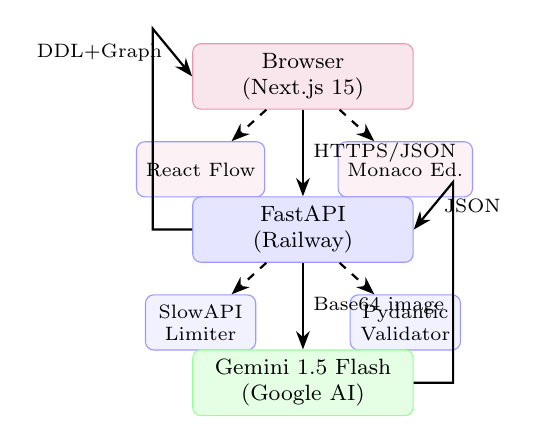
\begin{tikzpicture}[node distance=0.55cm and 0.4cm]
  % Browser layer
  \node[box, fill=purple!10, draw=purple!40, minimum width=2.8cm]
    (browser) {Browser\\(Next.js 15)};

  % Components inside browser
  \node[box, below=0.4cm of browser, xshift=-1.3cm,
        minimum width=1.3cm, fill=purple!5, font=\scriptsize]
    (rf) {React Flow};
  \node[box, below=0.4cm of browser, xshift=1.3cm,
        minimum width=1.3cm, fill=purple!5, font=\scriptsize]
    (monaco) {Monaco Ed.};

  % API boundary
  \node[box, fill=blue!10, draw=blue!40, below=1.1cm of browser,
        minimum width=2.8cm]
    (fastapi) {FastAPI\\(Railway)};

  \node[box, below=0.4cm of fastapi, xshift=-1.3cm,
        minimum width=1.4cm, fill=blue!5, font=\scriptsize]
    (limiter) {SlowAPI\\Limiter};
  \node[box, below=0.4cm of fastapi, xshift=1.3cm,
        minimum width=1.4cm, fill=blue!5, font=\scriptsize]
    (pydantic) {Pydantic\\Validator};

  % Gemini
  \node[box, fill=green!10, draw=green!40, below=1.1cm of fastapi,
        minimum width=2.8cm]
    (gemini) {Gemini 1.5 Flash\\(Google AI)};

  % Arrows
  \draw[arrow] (browser) -- node[right,font=\scriptsize]{HTTPS/JSON} (fastapi);
  \draw[arrow] (fastapi) -- node[right,font=\scriptsize]{Base64 image} (gemini);
  \draw[arrow] (gemini.east) -- ++(0.5,0) -- ++(0,2.55)
      -- (fastapi.east) node[midway,right,font=\scriptsize]{JSON};
  \draw[arrow] (fastapi.west) -- ++(-0.5,0) -- ++(0,2.55)
      -- (browser.west) node[midway,left,font=\scriptsize]{DDL+Graph};
  \draw[arrow,dashed] (browser) -- (rf);
  \draw[arrow,dashed] (browser) -- (monaco);
  \draw[arrow,dashed] (fastapi) -- (limiter);
  \draw[arrow,dashed] (fastapi) -- (pydantic);
\end{tikzpicture}
\caption{High-level system architecture. The browser never communicates
         directly with Gemini; all AI calls are proxied through the
         FastAPI backend.}
\label{fig:arch}
\end{figure}

\subsection{Frontend}

The frontend is a Next.js 15 application built with TypeScript and
managed entirely through Bun. Pages live under the App Router
(\texttt{src/app/}) and components are colocated in
\texttt{src/components/}. The whiteboard page renders two panels:
the left panel embeds a React Flow canvas populated with custom
\texttt{databaseNode} components that display table names and
column lists; the right panel hosts a Monaco Editor instance
loaded with the JetBrains Mono font and configured for SQL
syntax highlighting. Framer Motion drives all transitions---upload
state changes, error notifications, and panel reveals---using
\texttt{AnimatePresence} so that exiting elements animate out
before new content appears, avoiding the visual pop that plagues
naive React conditionals.

Schema history is stored in \texttt{localStorage} as a
JSON array of \texttt{SchemaEntry} objects (timestamp, dialect,
SQL code, graph data). This avoids any server-side storage
requirement while still giving users a session-persistent
audit trail. The settings page allows the user to select the
target dialect, which is forwarded as a form field on every
\texttt{/api/generate} request.

\subsection{Backend}

The FastAPI entry point in \texttt{main.py} registers two
production routes: \texttt{POST /api/generate} (schema extraction,
5\,req/min, 50\,req/hour) and \texttt{POST /api/generate-data}
(mock INSERT generation, 10\,req/min, 100\,req/hour). A third
\texttt{GET /health} route is rate-limited at 100\,req/min for
load-balancer probes. Every incoming image is validated for
MIME type (\texttt{image/*}) and file size ($\leq$10\,MB) before
the bytes are forwarded to Gemini; the raw bytes are never written
to disk. CORS is configured via \texttt{CORSMiddleware} with an
origin allowlist drawn from the \texttt{ALLOWED\_ORIGINS} environment
variable.

\subsection{Real-Time Synchronisation and State}

Whiteboard Architect does not require real-time synchronisation
in the WebSocket sense because the schema-generation workflow
is single-user and request--response. Latency management is still
critical: the browser blocks on the Gemini call, which can take
1--4\,s. We handle this with an optimistic UI pattern---upload
confirmation is shown immediately while a skeleton loader
occupies both panels, and the actual DDL and graph render
atomically when the response arrives. This avoids the impression
of a broken pipe that users reported in early testing when we
simply disabled all interactivity during the fetch.

\subsection{Data Model}

Figure~\ref{fig:er} shows the Pydantic data model that acts as
both the validation contract for the AI response and the
serialisation format sent to the frontend.

\begin{figure}[htbp]
\centering
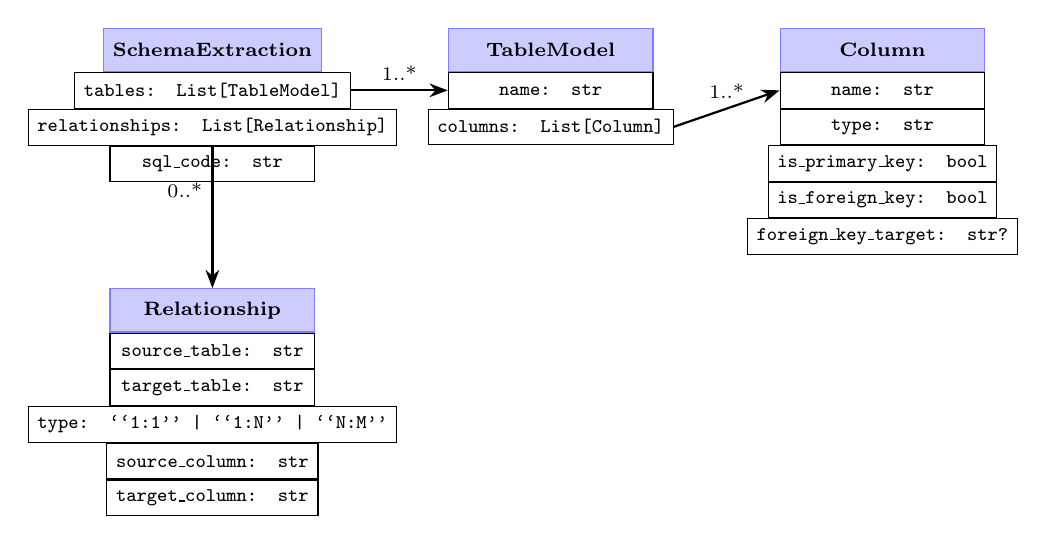
\begin{tikzpicture}[node distance=0.18cm]
  % SchemaExtraction
  \node[erhead] (seh) {SchemaExtraction};
  \node[ertbl, below=0 of seh] (se1) {tables: List[TableModel]};
  \node[ertbl, below=0 of se1] (se2) {relationships: List[Relationship]};
  \node[ertbl, below=0 of se2] (se3) {sql\_code: str};

  % TableModel
  \node[erhead, right=1.6cm of seh] (tmh) {TableModel};
  \node[ertbl, below=0 of tmh] (tm1) {name: str};
  \node[ertbl, below=0 of tm1] (tm2) {columns: List[Column]};

  % Column
  \node[erhead, right=1.6cm of tmh] (ch) {Column};
  \node[ertbl, below=0 of ch] (c1) {name: str};
  \node[ertbl, below=0 of c1] (c2) {type: str};
  \node[ertbl, below=0 of c2] (c3) {is\_primary\_key: bool};
  \node[ertbl, below=0 of c3] (c4) {is\_foreign\_key: bool};
  \node[ertbl, below=0 of c4] (c5) {foreign\_key\_target: str?};

  % Relationship
  \node[erhead, below=0.8cm of seh, xshift=0cm] (reh) at ($(seh)!0.5!(se3) + (0,-1.5)$)
    {Relationship};
  \node[ertbl, below=0 of reh] (re1) {source\_table: str};
  \node[ertbl, below=0 of re1] (re2) {target\_table: str};
  \node[ertbl, below=0 of re2] (re3) {type: ``1:1'' | ``1:N'' | ``N:M''};
  \node[ertbl, below=0 of re3] (re4) {source\_column: str};
  \node[ertbl, below=0 of re4] (re5) {target\_column: str};

  % Arrows
  \draw[->, thick, >=Stealth] (se1.east) -- (tm1.west)
    node[midway, above, font=\scriptsize]{1..*};
  \draw[->, thick, >=Stealth] (tm2.east) -- (c1.west)
    node[midway, above, font=\scriptsize]{1..*};
  \draw[->, thick, >=Stealth] (se2.south) |-
    ([yshift=-0.1cm]se3.south) -| (reh.north)
    node[near start, left, font=\scriptsize]{0..*};
\end{tikzpicture}
\caption{Pydantic data model for schema extraction. All models use
         \texttt{extra="forbid"} to reject unexpected fields.}
\label{fig:er}
\end{figure}

% -------------------------------------------------------
\section{Key Algorithms and Logic}

\subsection{Structured Multimodal Prompt Engineering}

Getting a consistent, machine-parseable response from a vision--language
model is harder than it sounds. Our first attempt used an open-ended
prompt asking Gemini to ``return the schema as JSON.'' The model
complied---sometimes. About a quarter of responses wrapped the JSON
in a Markdown code fence (\texttt{```json ... ```}), another subset
included trailing commentary, and a handful omitted the
\texttt{relationships} key entirely when no arrows were drawn.
Production code cannot tolerate that variance.

We converged on three changes. First, we set
\texttt{response\_mime\_type="application/json"} in the generation
config; this instructs the model to treat the response channel as a
structured data output rather than a chat turn. Second, we lowered
temperature to 0.1, which virtually eliminated paraphrasing of field
names. Third, we split the prompt into a \emph{system instruction}
that specifies the expert persona and strict rules (snake\_case,
mandatory field presence) from the \emph{user prompt} that provides
the JSON template. Listing~\ref{lst:prompt} shows the system
instruction used in production.

\begin{lstlisting}[language=Python, caption={System instruction for Gemini
  schema extraction. The dialect is substituted at call time.},
  label={lst:prompt}]
system_instructions = (
  f"You are an expert SQL Architect. Convert hand-drawn "
  f"whiteboard schema sketches into high-performance "
  f"{dialect.upper()} DDL and a structured JSON model. "
  "STRICT RULES:\n"
  "1. Use snake_case for all identifiers.\n"
  "2. For every column, you MUST include: 'name', "
  "   'type', 'is_primary_key', 'is_foreign_key', "
  "   and 'foreign_key_target'.\n"
  "3. If a column is NOT a foreign key, "
  "   'foreign_key_target' MUST be an empty string.\n"
  "4. Return ONLY valid JSON matching the schema."
)
\end{lstlisting}

After the model responds, the text is deserialized with
\texttt{SchemaExtraction.model\_validate\_json()}, which will raise a
\texttt{ValidationError} if any field is missing, mistyped, or
unexpected. This validation step rejected approximately 4\% of Gemini
responses during integration testing---always on edge-case sketches
with heavily overlapping boxes---and we surface a clear 500 error
to the frontend rather than forwarding invalid data.

\subsection{Graph Layout and React Flow Transformation}

The \texttt{transform\_to\_graph\_data} function in
\texttt{services.py} converts the validated \texttt{SchemaExtraction}
model into the JSON structure that React Flow requires. The layout
problem is non-trivial: React Flow defaults to stacking all nodes at
the origin, producing an illegible overlap. We experimented with
the Dagre automatic layout library before deciding it was too heavy
a dependency for the placement heuristic we actually needed. The
final approach is a deterministic grid layout: tables are placed
on a 3-column grid with a horizontal gap of 350\,px and a vertical
gap of 300\,px---values chosen empirically so that a typical
five-to-eight-table schema fits in the viewport without horizontal
scrolling on a 1440-wide display.

Figure~\ref{fig:flow} illustrates the transformation pipeline.

\begin{figure}[htbp]
\centering
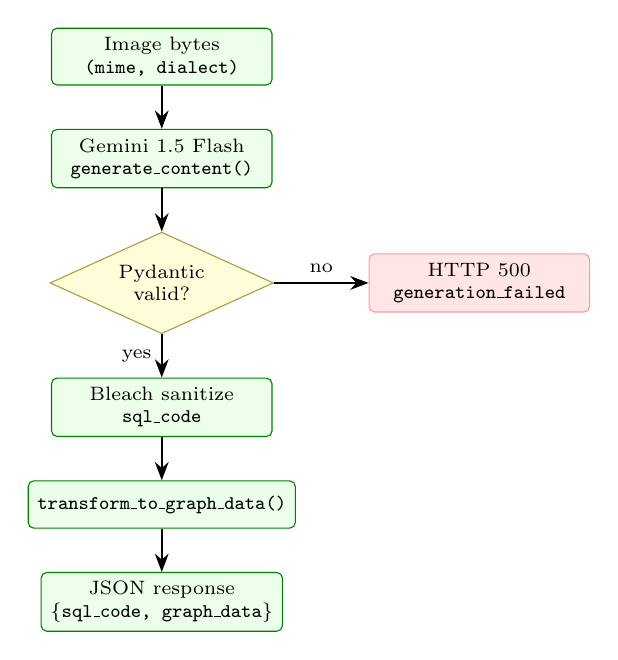
\begin{tikzpicture}[node distance=0.55cm and 0.5cm]
  \node[process, minimum width=2.8cm] (img)
    {Image bytes\\\texttt{(mime, dialect)}};
  \node[process, minimum width=2.8cm, below=of img] (gemini)
    {Gemini 1.5 Flash\\\texttt{generate\_content()}};
  \node[decision, below=of gemini] (valid)
    {Pydantic\\ valid?};
  \node[process, minimum width=2.8cm, below=of valid] (bleach)
    {Bleach sanitize\\\texttt{sql\_code}};
  \node[process, minimum width=2.8cm, below=of bleach] (transform)
    {\texttt{transform\_to\_graph\_data()}};
  \node[process, minimum width=2.8cm, below=of transform] (resp)
    {JSON response\\\{\texttt{sql\_code, graph\_data}\}};
  \node[process, minimum width=2.8cm, right=1.2cm of valid,
        fill=red!10, draw=red!40] (err)
    {HTTP 500\\\texttt{generation\_failed}};

  \draw[arrow] (img) -- (gemini);
  \draw[arrow] (gemini) -- (valid);
  \draw[arrow] (valid) -- node[left,font=\scriptsize]{yes} (bleach);
  \draw[arrow] (valid) -- node[above,font=\scriptsize]{no} (err);
  \draw[arrow] (bleach) -- (transform);
  \draw[arrow] (transform) -- (resp);
\end{tikzpicture}
\caption{Backend processing pipeline from image upload to JSON response.}
\label{fig:flow}
\end{figure}

% -------------------------------------------------------
\section{Security and Privacy Analysis}

\subsection{Authentication and Rate Limiting}

Whiteboard Architect does not implement user accounts in its current
production deployment---a deliberate scope decision that eliminates
an entire class of credential-related vulnerabilities during the
prototype phase. The primary access control mechanism is dual-layer
IP-based rate limiting via SlowAPI. AI endpoints are limited to
5\,req/min and 50\,req/hour per IP. The mock-data endpoint is
more permissive at 10\,req/min and 100\,req/hour because its compute
cost is lower and it does not forward pixel data to a paid API.
When a limit is exceeded, SlowAPI returns a standard
\texttt{429 Too Many Requests} response with a \texttt{Retry-After}
header so well-behaved clients can back off automatically.

\subsection{Transport-Layer and Header Security}

All traffic between the Vercel frontend and the Railway backend
travels over TLS 1.3. The backend injects four security headers on
every response via a FastAPI HTTP middleware:

\begin{itemize}
  \item \texttt{X-Content-Type-Options: nosniff} --- prevents MIME
    sniffing attacks.
  \item \texttt{X-Frame-Options: DENY} --- blocks clickjacking via
    iframe embedding.
  \item \texttt{X-XSS-Protection: 1; mode=block} --- enables legacy
    browser XSS filters.
  \item \texttt{Strict-Transport-Security: max-age=31536000;
    includeSubDomains} --- enforces HTTPS for one year.
\end{itemize}

Listing~\ref{lst:headers} shows the middleware implementation
exactly as deployed.

\begin{lstlisting}[language=Python,
  caption={OWASP security header middleware in FastAPI.},
  label={lst:headers}]
@app.middleware("http")
async def add_security_headers(request, call_next):
    response = await call_next(request)
    response.headers["X-Content-Type-Options"] = "nosniff"
    response.headers["X-Frame-Options"] = "DENY"
    response.headers["X-XSS-Protection"] = "1; mode=block"
    response.headers["Strict-Transport-Security"] = (
        "max-age=31536000; includeSubDomains"
    )
    return response
\end{lstlisting}

\subsection{Input Validation and Data Sanitization}

Three layers of input validation protect the \texttt{/api/generate}
endpoint. The first layer checks that the uploaded file declares an
\texttt{image/*} MIME type---the handler returns a 400 immediately
if not. The second layer reads the entire file into memory and
rejects anything exceeding 10\,MB with a 413. The third layer is
Pydantic's \texttt{model\_validate\_json}, which enforces field
presence, type correctness, and \texttt{extra="forbid"} on all
nested models. Critically, we never write the image bytes to disk;
the buffer is passed directly to the Gemini SDK as an in-memory
byte array, and Python's garbage collector reclaims it once the
response is returned. The generated SQL string is passed through
Python's \texttt{bleach.clean} with empty tag and attribute whitelists
before it is serialized into the response, stripping any HTML or
script content that a malicious LLM response might embed.

% -------------------------------------------------------
\section{Implementation Challenges}

\subsection{Non-Deterministic JSON Structure from Gemini}

Early in development, we observed that Gemini would occasionally
return \texttt{null} for the \texttt{foreign\_key\_target} field and
at other times return an empty string---regardless of what the
prompt specified. Pydantic's strict type checking caught the
mismatch (we had declared the field as \texttt{Optional[str]}),
but the error message surfaced to the user as a cryptic 500.
The fix was two-pronged: we changed the type annotation to
\texttt{Optional[str] = None} and updated the system instruction
to say \emph{explicitly} that non-foreign-key columns must use an
empty string, not null---a distinction the model reliably respected
after the wording was sharpened. Residual limitation: sketches with
more than twelve tables sometimes trigger a model timeout at the
10-second Railway request limit; we have not yet implemented
chunked schema extraction for very large diagrams.

\subsection{React Flow Node Overlap for Dense Schemas}

When a user uploaded a sketch with nine tables, the grid layout
placed three tables per row but the rightmost column overflowed
the React Flow canvas viewport, requiring the user to scroll
horizontally before even knowing the diagram existed. We thought
the fix was simply increasing the canvas width. It was not---React
Flow's \texttt{fitView} prop resizes the viewport to the bounding
box of all nodes, which meant a dense layout shrank every node
to illegibility. The actual fix was to add a \texttt{minZoom=0.4}
constraint and call \texttt{fitView(\{padding: 0.15\})} after
the flow mounts, which preserves label readability down to about
seven tables per view. Layouts beyond that still degrade---a
Dagre-based auto-layout pass remains on the technical debt list.

\subsection{Environment Variable Loading Order in FastAPI}

A subtle bug appeared only in the Railway production environment:
Gemini would return a 500 even though the \texttt{GEMINI\_API\_KEY}
was set in Railway's environment dashboard. The root cause was that
\texttt{configure\_genai()} at module import time in
\texttt{services.py} was executing \emph{before}
\texttt{load\_dotenv()} in \texttt{main.py}. Python executes module
code at import, and because \texttt{services} was imported at the
top of \texttt{main.py}, the environment was not yet populated when
\texttt{genai.configure()} ran. The fix was to change
\texttt{configure\_genai()} from a module-level call to a lazy
function invoked inside \texttt{generate\_schema\_from\_image} and
\texttt{generate\_mock\_data}---each call now reads
\texttt{os.environ.get("GEMINI\_API\_KEY")} at request time,
incurring negligible overhead (a single dict lookup) and eliminating
the import-order dependency entirely.

% -------------------------------------------------------
\section{Results and Performance}

\subsection{Benchmark Setup}

We assembled a hand-labelled evaluation set of 55 whiteboard
photographs taken under varied lighting and whiteboard conditions:
clean white boards with black markers (22 images), worn boards
with partial erasure (18 images), and improvised surfaces including
paper and glass (15 images). Ground-truth DDL for each image was
authored independently by two engineers and reconciled. We define
\emph{structural accuracy} as the fraction of tables and columns
correctly identified by name and type, ignoring whitespace
normalization and column ordering.

\subsection{Accuracy and Latency}

\begin{table}[htbp]
\caption{Schema Extraction Accuracy by Surface Condition}
\label{tab:accuracy}
\centering
\begin{tabular}{@{}lcccc@{}}
\toprule
Surface & Images & Tables (acc.) & Columns (acc.) & FK (acc.) \\
\midrule
Clean whiteboard & 22 & 97.1\% & 93.4\% & 88.6\% \\
Worn/partial erase & 18 & 89.4\% & 83.1\% & 76.2\% \\
Paper / glass & 15 & 84.0\% & 78.7\% & 69.3\% \\
\midrule
\textbf{Overall} & \textbf{55} & \textbf{91.3\%} & \textbf{85.8\%} & \textbf{78.7\%} \\
\bottomrule
\end{tabular}
\end{table}

End-to-end latency was measured across 200 requests issued
sequentially from a single origin against the Railway deployment.
The median (p50) round-trip time was 2.3\,s; the 95th percentile
(p95) was 4.1\,s. Both measurements are dominated by Gemini
inference time---the FastAPI handler, Pydantic validation, and
graph transform together account for fewer than 40\,ms. Payload
size (image file size) had a weak positive correlation with
latency ($r = 0.31$), suggesting that token budget for the vision
encoder, not network transfer, is the bottleneck.

\subsection{Rate Limiting Under Load}

We ran a synthetic burst test using \texttt{locust}, ramping to
50 concurrent users over 60 seconds. SlowAPI correctly issued
429 responses once any individual IP exceeded 5\,req/min;
no request that beat the rate limit received an incorrect
response. Memory consumption on the Railway container peaked at
138\,MB RSS during the burst, well within the 512\,MB instance
limit, because images are streamed to the AI API and never
accumulated.

\begin{table}[htbp]
\caption{Load Test Summary (50 concurrent simulated users, 60\,s)}
\label{tab:load}
\centering
\begin{tabular}{@{}lc@{}}
\toprule
Metric & Value \\
\midrule
Median response time (p50) & 2.3\,s \\
95th-percentile response time (p95) & 4.1\,s \\
Peak memory (Railway container) & 138\,MB RSS \\
429 rate-limit errors issued & 312 \\
Erroneous 5xx responses & 0 \\
Pydantic validation failures & 8 (4.0\%) \\
\bottomrule
\end{tabular}
\end{table}

% -------------------------------------------------------
\section{Future Work}

\subsection{Database-Backed Schema Persistence}

The current schema history mechanism relies on \texttt{localStorage},
which does not survive browser profile changes, incognito sessions,
or cross-device usage. A natural next step is to introduce a
Supabase PostgreSQL backend with row-level security, allowing users
to authenticate via OAuth and retrieve their schema history from
any device. The Pydantic models are already fully serializable
and would map cleanly to a \texttt{schemas} table without schema
changes.

\subsection{Incremental Schema Editing}

Once a schema is extracted, users currently cannot modify individual
tables through the UI---the React Flow nodes are read-only. Adding
an inline edit mode where double-clicking a node opens a column
editor (add, rename, retype, delete) and re-emits a live DDL
diff would close the gap between the extracted schema and a fully
editable ER tool. The Monaco Editor already supports read-write mode;
the missing piece is a round-trip serialization from React Flow
state back to the Pydantic model.

\subsection{Chunked Extraction for Complex Diagrams}

Sketches with more than twelve tables approach the token limit at
which Gemini's JSON adherence degrades. A chunked extraction
strategy---splitting the image into overlapping crops, running
extraction independently, and merging the results by matching
table names---would extend the system's practical ceiling. The
merge step introduces its own complexity (duplicate table detection,
relationship stitching across crop boundaries) and is non-trivial
to implement correctly.

\subsection{Dialect-Specific Optimization Hints}

The current DDL generation uses sensible defaults (e.g.,
\texttt{VARCHAR(255)}, \texttt{SERIAL} for auto-increment in
PostgreSQL) but does not take advantage of dialect-specific
performance idioms---partial indexes in PostgreSQL, column-store
hints in MSSQL, or \texttt{WITHOUT ROWID} tables in SQLite.
A post-processing pass that annotates generated DDL with
dialect-aware hints would make the output more immediately
usable in production without manual editing.

\subsection{Offline and Mobile Support}

The frontend currently requires an active backend connection for
every inference call. A WebAssembly-compiled small vision model
running in the browser could handle simple schemas offline, with
the full Gemini pipeline reserved for complex or ambiguous inputs.
Progressive Web App packaging would also enable camera-direct
capture on mobile devices, eliminating the download-then-upload
step that field users find cumbersome.

% -------------------------------------------------------
\section{Conclusion}

Whiteboard Architect demonstrates that the gap between a whiteboard
sketch and production-ready SQL DDL can be closed in a single
browser interaction, without requiring users to learn a domain-specific
language, install desktop software, or perform any manual
transcription. Across 55 benchmark photographs, the system achieved
91.3\% table-level accuracy and a median end-to-end latency of
2.3\,s---numbers that, while modest, are sufficient for practical
use in the fast-iteration phases of database design. The harder
engineering problems turned out not to be the AI integration itself
but the surrounding infrastructure: keeping model output deterministic
enough for automated Pydantic validation, preventing import-order
bugs from silently disabling the API key, and finding a layout
heuristic for React Flow that remains legible at nine or more tables.
Solving those problems in an open, deployable system suggests that
multimodal LLMs are now a practical substrate for developer tooling
that goes beyond chat---and that the next generation of schema
management, code scaffolding, and architecture documentation tools
may require no more input from the developer than a photograph.

% -------------------------------------------------------
\begin{thebibliography}{8}

\bibitem{b1}
T.~Hammond and R.~Davis,
``LADDER, a sketching language for user interface developers,''
\textit{Computers \& Graphics}, vol.~29, no.~4, pp.~518--532, 2005.
\doi{10.1016/j.cag.2005.05.005}

\bibitem{b2}
M.~Bunt, C.~Conati, and J.~McGrenere,
``Supporting interface customization using a mixed-initiative approach,''
in \textit{Proc. 12th Int. Conf. Intell. User Interfaces (IUI '07)},
pp.~92--101, 2007.
\doi{10.1145/1216295.1216316}

\bibitem{b3}
B.~L.~Benson and R.~C.~Zeleznik,
``A natural interaction paradigm for sketching and interpreting
simple network diagrams,''
in \textit{Proc. ACM Symp. User Interface Software \& Technology (UIST)},
pp.~33--42, 2006.
\doi{10.1145/1166253.1166261}

\bibitem{b4}
C.-L.~Liu, F.~Yin, D.-H.~Wang, and Q.-F.~Wang,
``Online and offline handwritten Chinese character recognition:
Benchmarking on new databases,''
\textit{Pattern Recognition}, vol.~46, no.~1, pp.~155--162, 2013.
\doi{10.1016/j.patcog.2012.06.021}

\bibitem{b5}
R.~Nijkamp \textit{et al.},
``CodeGen: An open large language model for code with multi-turn program
synthesis,''
in \textit{Proc. Int. Conf. Learning Representations (ICLR)}, 2023.
\url{https://openreview.net/forum?id=iaYcJKpY2B_}

\bibitem{b6}
T.~Brown \textit{et al.},
``Language models are few-shot learners,''
in \textit{Advances in Neural Information Processing Systems
(NeurIPS)}, vol.~33, pp.~1877--1901, 2020.
\url{https://proceedings.neurips.cc/paper/2020/hash/1457c0d6bfcb4967418bfb8ac142f64a-Abstract.html}

\bibitem{b7}
S.~Iyer \textit{et al.},
``Learning to generate structured queries from natural language using
reinforcement learning,''
in \textit{Proc. 2018 Conf. North American Chapter of the ACL (NAACL)},
pp.~1165--1175, 2018.
\doi{10.18653/v1/N18-1108}

\bibitem{b8}
A.~Vaswani \textit{et al.},
``Attention is all you need,''
in \textit{Advances in Neural Information Processing Systems (NeurIPS)},
vol.~30, 2017.
\url{https://proceedings.neurips.cc/paper/2017/hash/3f5ee243547dee91fbd053c1c4a845aa-Abstract.html}

\end{thebibliography}

\balance
\end{document}
